\subsection{Phasenschieber} % (fold)
\label{sub:Phasenschieber}
\begin{frame}
\frametitle{Phsenscheiber}
\framesubtitle{}
    \begin{block}{Phasenschieber}
         \begin{figure}[H]
         \begin{center}
                 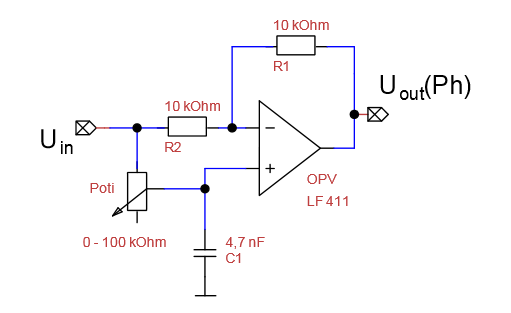
\includegraphics[scale=0.4]{./img/schaltung/Phasenschieber.png}
         \end{center}
         \end{figure}
         \begin{itemize}
             \item Verschiebung der Phase $U = e^{-i\omega} \rightarrow e^{-i
             \omega + \varphi}$ in Abhängigkeit vom Potentiometer $R_{pot}$
         \end{itemize}
    \end{block}
\end{frame}
\begin{frame}
\frametitle{Phsenscheiber}
\framesubtitle{}
    \begin{columns}[c]
        \column{0.7\textwidth} 
        \begin{block}{Funktionsweise}
         \begin{itemize}
            \item Aus Vorbereitung wissen wir:
            \begin{equation*}
                U_{out} \approx \underbrace{\frac{1-if2\pi R_{poti}
                C}{1+if2\pi R_{poti}}}_{|\cdot| = 1}
                \cdot U_{in} 
            \end{equation*}
            \begin{equation*}
                \varphi = \arctan \left( \frac{2C R_{poti} f 2\pi}{1 - C^2
                R_{poti}^2 (f2\pi)^2} \right)
            \end{equation*}
         \end{itemize}
        \end{block}
        \column{0.3\textwidth} 
         \begin{figure}[H]
         \begin{center}
                 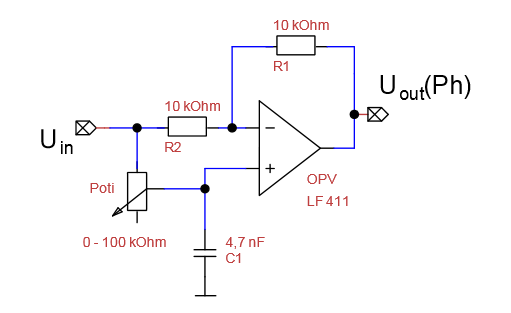
\includegraphics[scale=0.3]{./img/schaltung/Phasenschieber.png}
         \end{center}
         \end{figure}
    \end{columns}
\end{frame}

\begin{frame}
\frametitle{Phsenscheiber}
\framesubtitle{}
    \begin{columns}[c]
        \column{0.5\textwidth} 
         \begin{figure}[H]
         \begin{center}
                 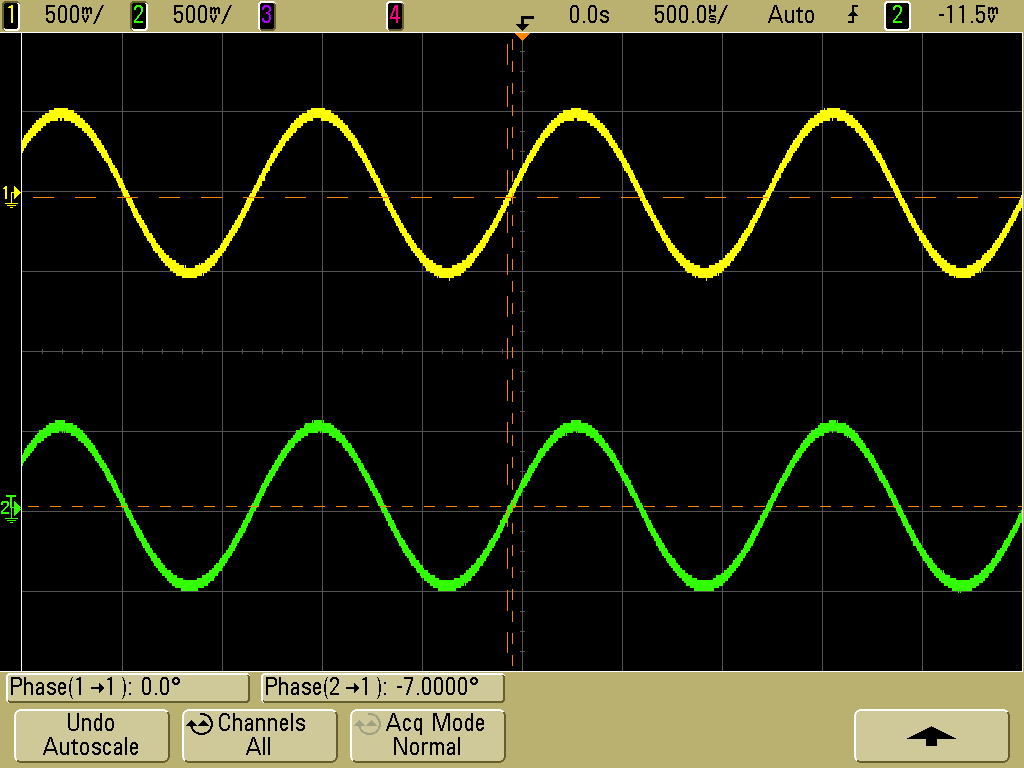
\includegraphics[scale=0.15]{./img/oszi/scope_0.png}
         \end{center}
         \caption{$\varphi = 0 ^{\circ}$}
         \end{figure}
        \column{0.5\textwidth} 
         \begin{figure}[H]
         \begin{center}
                 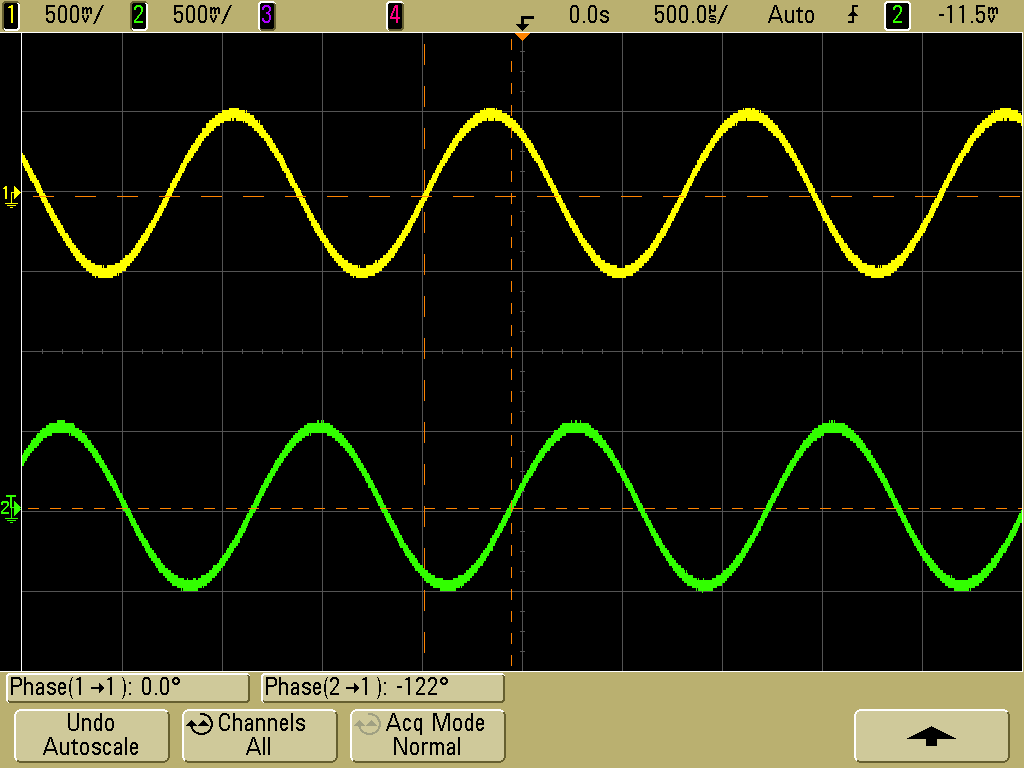
\includegraphics[scale=0.15]{./img/oszi/scope_5.png}
         \end{center}
         \caption{$\varphi= 130 ^{\circ}$}
         \end{figure}
    \end{columns}
\end{frame}

\begin{frame}
\frametitle{Phasenschieber}
\framesubtitle{}
    \begin{columns}[c]
        \column{0.25\textwidth} 
        \boxed{
        \begin{tabular}{c|c}
            $R_{poti} / k\Omega$ & $\varphi / ^{\circ}$ \\
            \hline
            $6.18$&$17$ \\
            $16.8$&$43$ \\
            $23.8$&$57$ \\
            $42.38$&$90$ \\
            $71.2$&$120$ 
        \end{tabular}  
            }
        \column{0.7\textwidth} 
        \begin{figure}[H]
        \begin{center}
                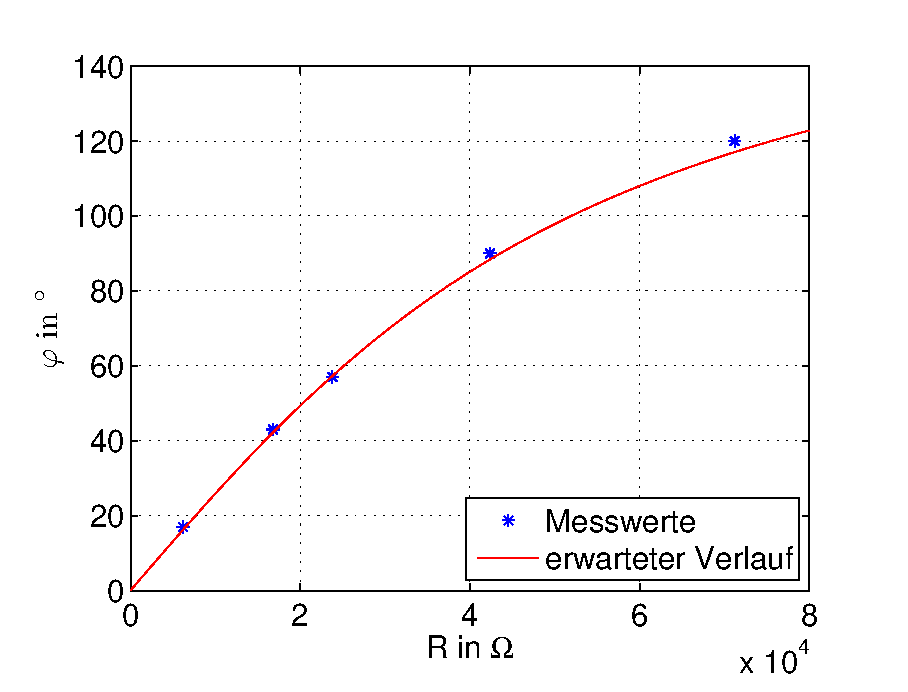
\includegraphics[scale=0.6]{./img/plots/Auf_1_a.eps}
        \end{center}
        \end{figure}
    \end{columns}
\end{frame}

\begin{frame}
\frametitle{Phasenschieber}
\framesubtitle{Funktioniert der Phasenschieber auch für andere Signalformen?}
    \begin{columns}[c]
        \column{0.5\textwidth}    
        \begin{figure}[H]
        \begin{center}
                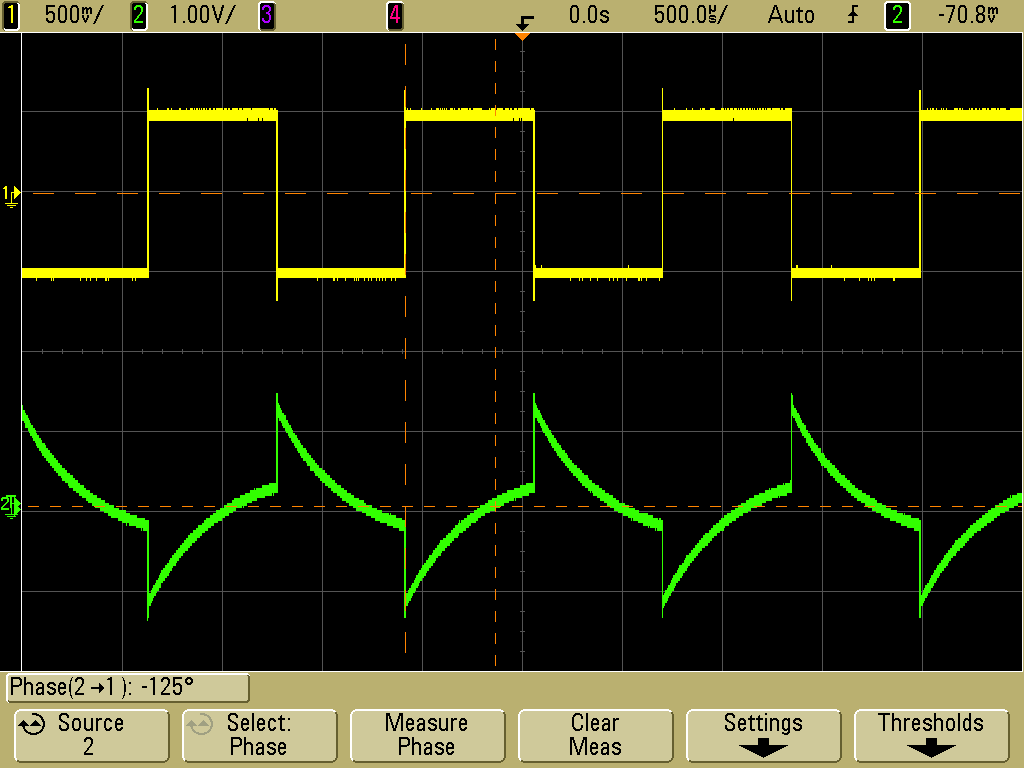
\includegraphics[scale=0.15]{./img/oszi/scope_10.png}
        \end{center}
        \caption{Rechtecksspannung}
        \end{figure}
        \column{0.5\textwidth}    
        \begin{figure}[H]
        \begin{center}
                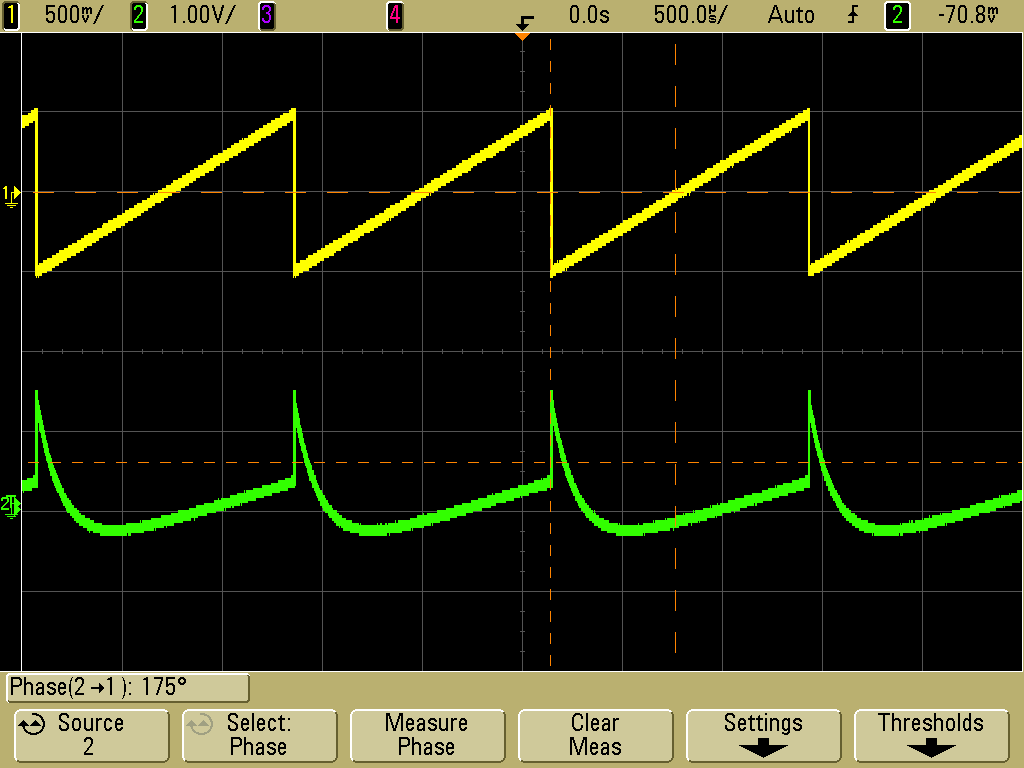
\includegraphics[scale=0.15]{./img/oszi/scope_12.png}
        \end{center}
        \caption{Dreicksspannung}
        \end{figure}
    \end{columns}
\end{frame}

\begin{frame}
\frametitle{Phasenschieber}
\framesubtitle{Funktioniert der Phasenschieber auch für andere Signalformen?}
    \begin{columns}[c]
        \column{0.5\textwidth}    
        \begin{figure}[H]
        \begin{center}
                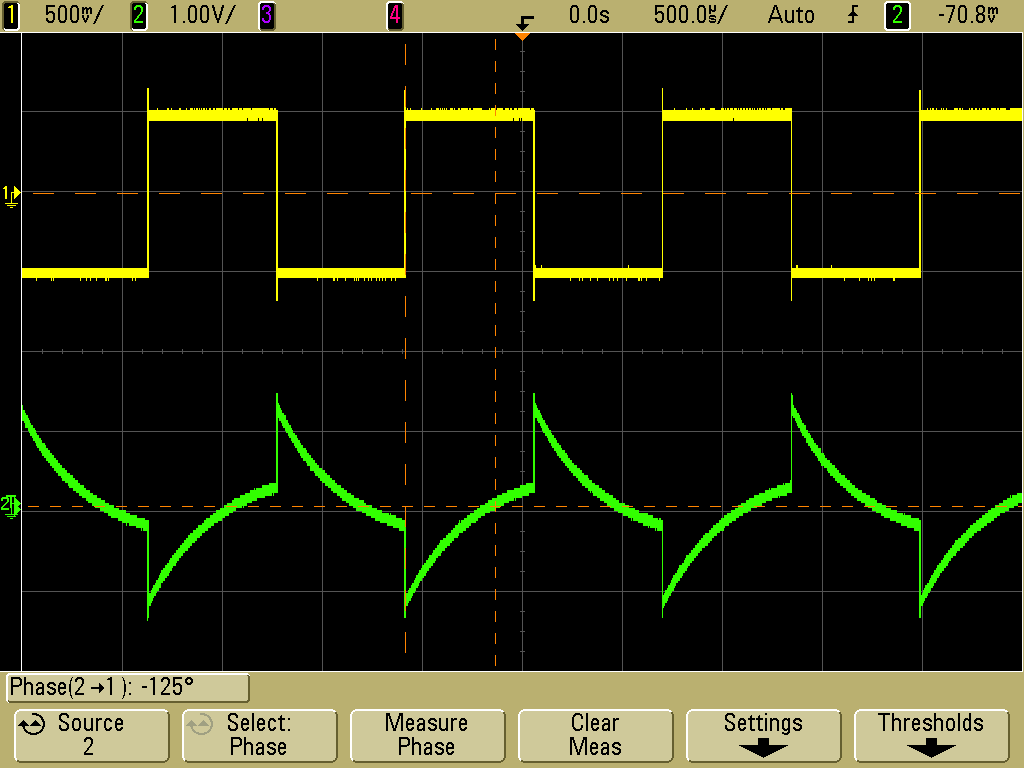
\includegraphics[scale=0.1]{./img/oszi/scope_10.png}
        \end{center}
        \end{figure}
        \column{0.5\textwidth}    
        \begin{figure}[H]
        \begin{center}
                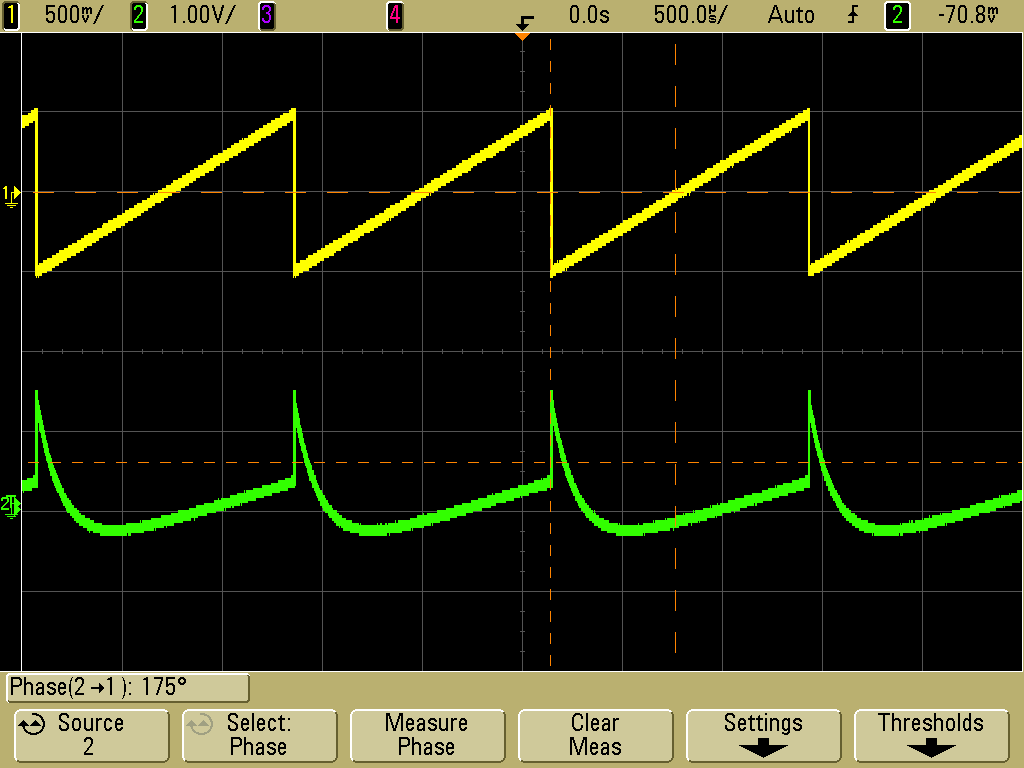
\includegraphics[scale=0.1]{./img/oszi/scope_12.png}
        \end{center}
        \end{figure}
    \end{columns}
    \begin{block}{Erklärung}
        ??? 
    \end{block}
\end{frame}
% subsection Phasenschieber (end)

